\section{House Manager}

Una vez descritos todos los componentes gráficos necesarios para realizar la aplicacion se desarrollaron todos los objetos necesarios para implementar los requerimientos descritos en la hoja "requerimientos funcionales" del formato RUP \ref{tab0}. La aplicacion fue desarrollada utilizando el paradigma MVC, para ello, se organizo el proyecto en 3 carpetas principalmente; view, control y model, donde todos los componentes y scripts son gestionados desde un archivo principal. Debido a la naturaleza grafica del proyecto y las limitaciones tecnicas del hardware raspberry, se utilizo Python 2.7 para garantizar la compatibilidad de la mayor cantidad de sistemas operativos y librerias. 
Para el desarrollo de la aplicacion fueron utilizadas las siguientes librerias: 
\begin{itemize}
	\item paho-mqtt: Esta libreria se utilizó para establecer la comunicación con el broker de mqtt nativo de Google cloud iot.
	\item numpy, scipy: Estas listrerias fueron utilizadas para facilitar el procesamiento de vectores y mejorar el tiempo de procesamiento de los mismos.
	\item pyqtgraph: Fue utilizada para gestionar y renderizar las gráficas con un valor optimo de fotogramas por segundo
	\item pyqtgraph: Fue utilizada para gestionar y renderizar las gráficas con un valor optimo de fotogramas por segundo
	\item: http.client: Esta libreria fue utilizada para establecer una comunicacion basada en solicitudes http con un "endpoint" del backend
	\item: pyjwt cryptography: Con esta libreria se desarrolló la etapa de encriptacion de datos adicional basada en Java Web Tokens.	
\end{itemize}

Dentro de la carpeta del proyecto se pueden encontrar scripts que fueron importantes para el despliegue de la aplicacion. Por ejemplo; en el directorio "./src/installing/" se encuentran los ejecutables para la instalacion de la aplicacion en windows y debian; en el directorio "./src/test/" se encuentran las rutinas de testing utilizadas para algunas rutinas y objetos utilizados en el programa.

Pensando en la escalabilidad del sistema, se definio un espacio para las "aplicaciones" adicionales donde se pudieran incluir nuevas rutinas de adquisicion y control para dispositivos nuevos \ref{fig_6}. Como prueba de concepto se utilizo una rutina serial para adquirir el valor de khw acumulado en un contador electrico bifasico Inelca. Respecto a esta consideracion de diseño se hablara mas en proximos apartados

\begin{figure}[htbp]
	\centerline{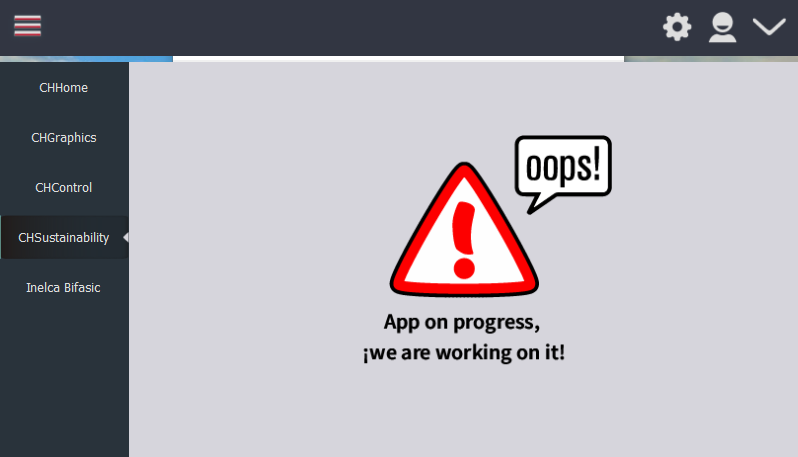
\includegraphics[width=8.5cm]{figuras/housemanager_newapp.png}}
	\caption{Visualizacion de la escalabilidad del sistema con una app no desarrollada por completo}
	\label{fig_6}
\end{figure}

En adicion, se diagramo la experiencia de usuario de tal forma que el control y la medicion de los dispositivos conectados a la tarjeta tuvieran el mismo "costo de interacción", es decir, que ambos estuvieran a la misma cantidad de clicks desde cualquier ventana del sistema. Por ende, todas las aplicaciones adicionadas en versiones futuras le seran mas faciles de asimilar al usuario.

\subsection{Requerimientos Funcionales}

Durante la etapa de conceptualizacion del proyecto de ingeniería que este documento describe se utilizó una herramienta de planeación llamada RUP; con un documento llamado "Requerimientos funcionales", dentro de los requerimientos implementados descritos en ese documento estan: 

\begin{figure}[htbp]
	\centerline{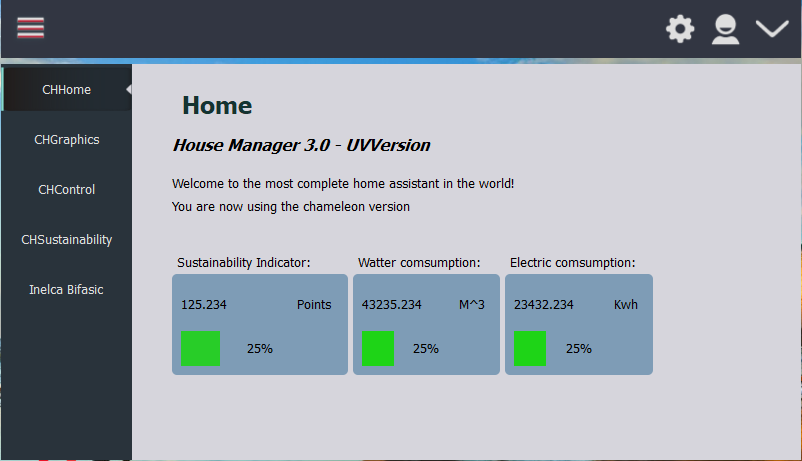
\includegraphics[width=8.5cm]{figuras/housemanager_home.png}}
	\caption{Escena del home del House Manager con barras de progresso para la indicacion dinamica}
	\label{fig_7}
\end{figure}

\begin{enumerate}
	\item \textsl{"El sistema debe mostrar graficamente la cantidad de agua y potencia consumida durante el dia contrastandolas con un valor maximo recomendado":} Para el desarrollo de esta funcionalidad se utilizó un componente grafico tipo barra de progreso donde su 100 porciento tenia como referencia la cantidad de agua recomendada para el numero de personas presentes en la vivienda\ref{fig_7}. El numero de personas presentes en la vivienda fue un dato ingresado manualmente por configuracion inicial (sobre el sistema de configuracion se hablara en los siguientes apartados de este capitulo)
	
	\item \textsl{"Por defecto el uso de las cargas electricas más significativas debe programarse surante los picos de generacion en la casa, estos horarios podran ser modificados bajo una advertencia de uso no eficiente":} En miras de implementar esta funcionalidad se utilizo un elemento grafico tipo calendario para configurar de manera individual las ventanas de activación de las cargas electricas en la vivienda\ref{fig_8}. 
	También, se consideró la opcion de activacion o desactivacion inmediata de los circuitos; para ello se, implementó una rutina flexible que permitio ignorar las cargas electricas que el usuario habia modificado manualmente (Esta rutina se nombro "Scheduler Handler"), lo anterior unicamente durante 24 horas para no afectar el objetivo de sostenibilidad de la vivienda. 
	En adicion, se utilizo la conexion mqtt para accionar remotamente cualquiera de los circuitos localmente gestionados, en caso de recibir un mensaje de control para los circuitos el sistema tambien suspendiera por 24 horas la accion del "Schedule Handler".
	
	\item: \textsl{"El sistema debe poder comunicarse con una base de datos que represente todas las variables y el estado de los circuitos de la vivienda":} Para la implementacion de este requeirmiento se creo un "endpoint" en el servicio de backend con la capacidad de hacer consultas de historicos a la base de datos. La solución tiene este comportamiento puesto que la aplicacion del cliente finl no debe tener ningun tipo de credencial para el acceso a la informacion directmente, con una capa de procesamiento se pueden integrar este tipo de solicitudes con el mismo sistema de encriptacion del broker de mqtt (para más informacion de los endpoints y la rutina de encriptacion vease el capitulo "Backend").
\end{enumerate}


\begin{figure}[htbp]
	\centerline{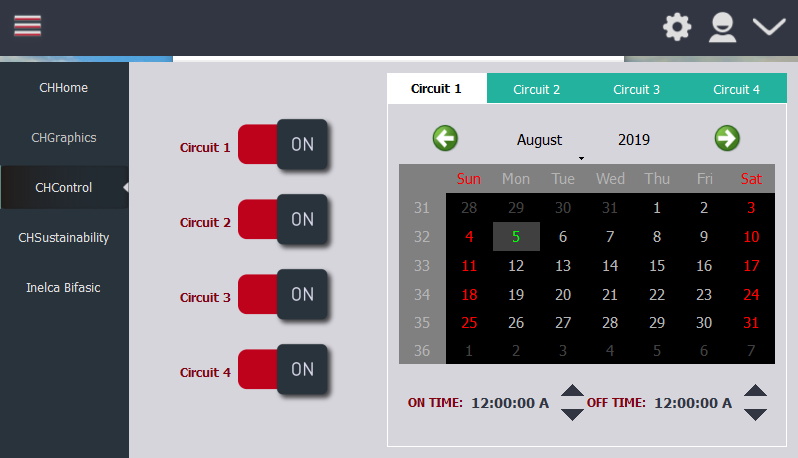
\includegraphics[width=8.5cm]{figuras/housemanager_control.png}}
	\caption{Escena de control del House Managern con sus calendarios}
	\label{fig_8}
\end{figure}

\subsection{Funciones adicionales}

En adición a los requerimientos funcionales, se añadieron funciones a la conceptualización de diseño original para mejorar el funcionamiento de la plataforma y la experiencia de usuario. Dentro de estas funciones podemos encontrar la configuracion del sistema, la posibilidad de guardar localmente para no perder la informacion adquirida, etc. 
Para comprender mejor estas funciones adicionales, seran descritas a continuacion:


\begin{enumerate}
	\item \textbf{Handler remoto:} Esta caracteristica le permite al sistema cambiar de manera automatica entre el modo remoto y el modo local para no perder información en ningun momento de la adquisicion. En caso de la caida repentina de la red es capaz de cambiar al modo local sin la perdida de ningun dato. Tambien, es capaz de entender cuando el usuario desea que el dispositivo funcione permanentemente de manera local.
	
	\item \textbf{Sistema de almacenamiento local:} Con esta caracteristica el House Manager puede almacenar todos los datos adquiridos en una hoja de excel generando archivos organizados por dias. Tambien es capaz de almacenar en un archivo diferentee los datos presentes en la gráfica en cuestion\ref{fig_9}.
	
	\item \textbf{Ajustes de configuracion} Esta es una caracteristica que incluye una ventana adicional donde se configuran los aspectos concernientes al sistema en general\ref{fig_10}. Los aspectos configurables del sistema son: La frecuencia en segundos con la que se reportan los datos al servidor, el costo del kilo watt hora, el costo del metro cubico de agua, el dia de notificacion del correo (ver funcion "Notificacion automatica"), el modo de funcionamiento (remoto o local) y el nombre de la ubicacion (este nombe es opcional y sirve para administrar los diferentes dispositivos).
	
	\item \textbf{Notificacion Automatica:} Para el correcto desarrollo de esta funcion se compró el dominio \href{www.alfagenos.com}{www.alfagenos.com} como remitente de las notifiacciones enviadas por correo, esta notificacion tendra lugar dependiendo de la configuracion establecida y notificara el gasto en pesos del consumo electrico y de agua hasta la fecha establecida en la configuracion.

	\item\textbf{Autenticación usando google:} Para desarrollar esta funcionalidad se utilizó la api de autenticacion de google y se creo una escena aparte para la visualizacion del usuario \ref{fig_11}.
	
	
	\item \textbf{Doble nivel de encriptacion:} Debido a las exigencias de los servidores de google se implementaron 2 capas de seguridad de encriptacion para la  comunicacion de la aplicacion con el backend. La primera capa es de tipo TLS y opera para cuaquier producto de google, inclusive las operaciones realizadas por los navegadores. La segunda se implemento usando encriptacion "RS256" a travez de JWT.
\end{enumerate}

\begin{figure}[htbp]
	\centerline{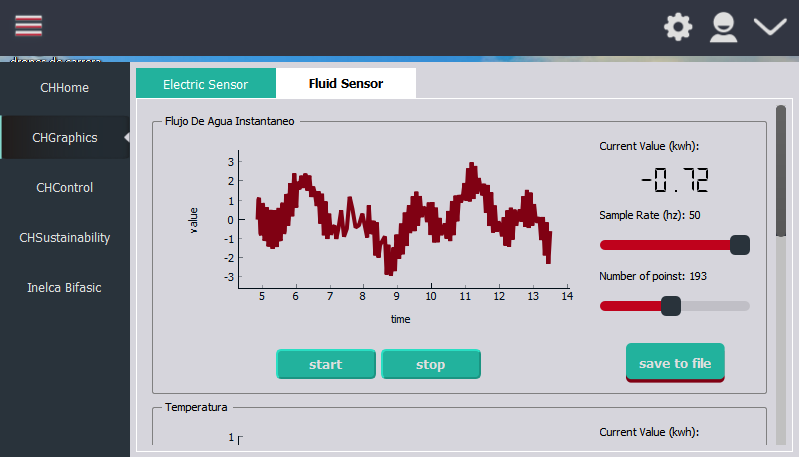
\includegraphics[width=8.5cm]{figuras/housemanager_measure.png}}
	\caption{Escena de medición del House Manager, con su respectivo panel para guardar los datos}
	\label{fig_9}
\end{figure}
 
 \begin{figure}[htbp]
 	\centerline{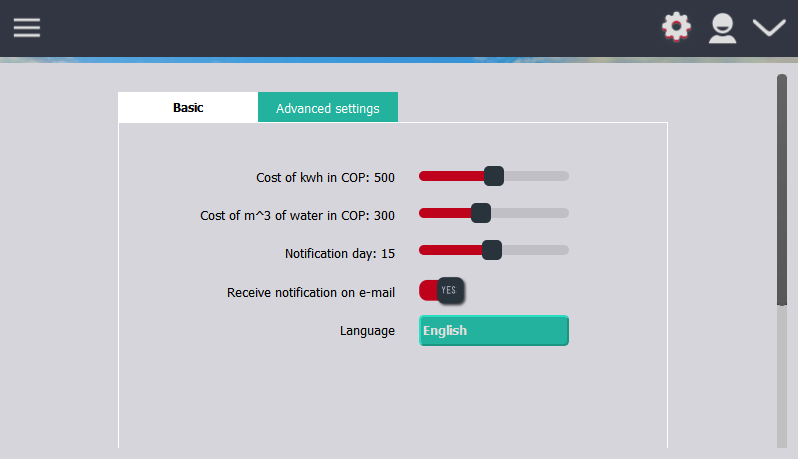
\includegraphics[width=8.5cm]{figuras/housemanager_config.png}}
 	\caption{Escena de configuracion del dispositivo House Manager}
 	\label{fig_10}
 \end{figure}
 
 \begin{figure}[htbp]
 	\centerline{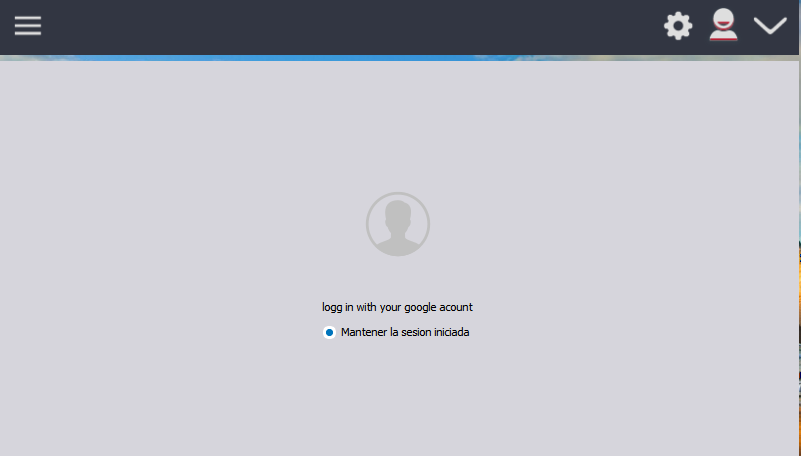
\includegraphics[width=8.5cm]{figuras/housemanager_user.png}}
 	\caption{Escena para el inicio de sesion del House Manager}
 	\label{fig_11}
 \end{figure}

 \subsection{Algoritmos Utilizados}
 
 **** preambulo pra hablar de los algoritmos utilizados en esta aplicacion y como representan threads en python. Mencionar la estructura de su funcion (reciben como informacion un puntero a su pariente mayor que en la mayoria de los casos es uno de los 3 elementos: Modelo, Vista o Controlador, que ocurren en segundo plano, es decir que no tienen un comportamiento muy determinista en el tiempo de ejecucion, etc.
 
 \subsubsection{Scheduler Handler}
 
 ***incluir diagrama del algoritmo y explicarlo 
 
  \subsubsection{Remote Mode Handler}
 
 ***incluir diagrama del algoritmo y explicarlo 
 
  \subsubsection{Mail Notification Handler}
 
 ***incluir diagrama del algoritmo y explicarlo 
 
   \subsubsection{Data Report Handler}
 
 ***incluir diagrama del algoritmo y explicarlo 
 
    \subsubsection{Indicator Handler}
 
 ***incluir diagrama del algoritmo y explicarlo 
 
 
